\chapter{2-D Convolutional Nerual Networks}
\label{3.2D_CNN}
\lhead{\emph{2-D Convolutional Neural Networks}}

Escribir algo de cabecera.
% TODO: ??
% TODO: ??


\section{Data preprocessing}
% TODO: Resizing
% TODO: Slicing
% TODO: Normalizing

\newpage
\section{U-Net}
Start writing about U-Net.

% TODO: Describe the model
% TODO: Training parameters

\begin{center}
\hspace*{15pt}
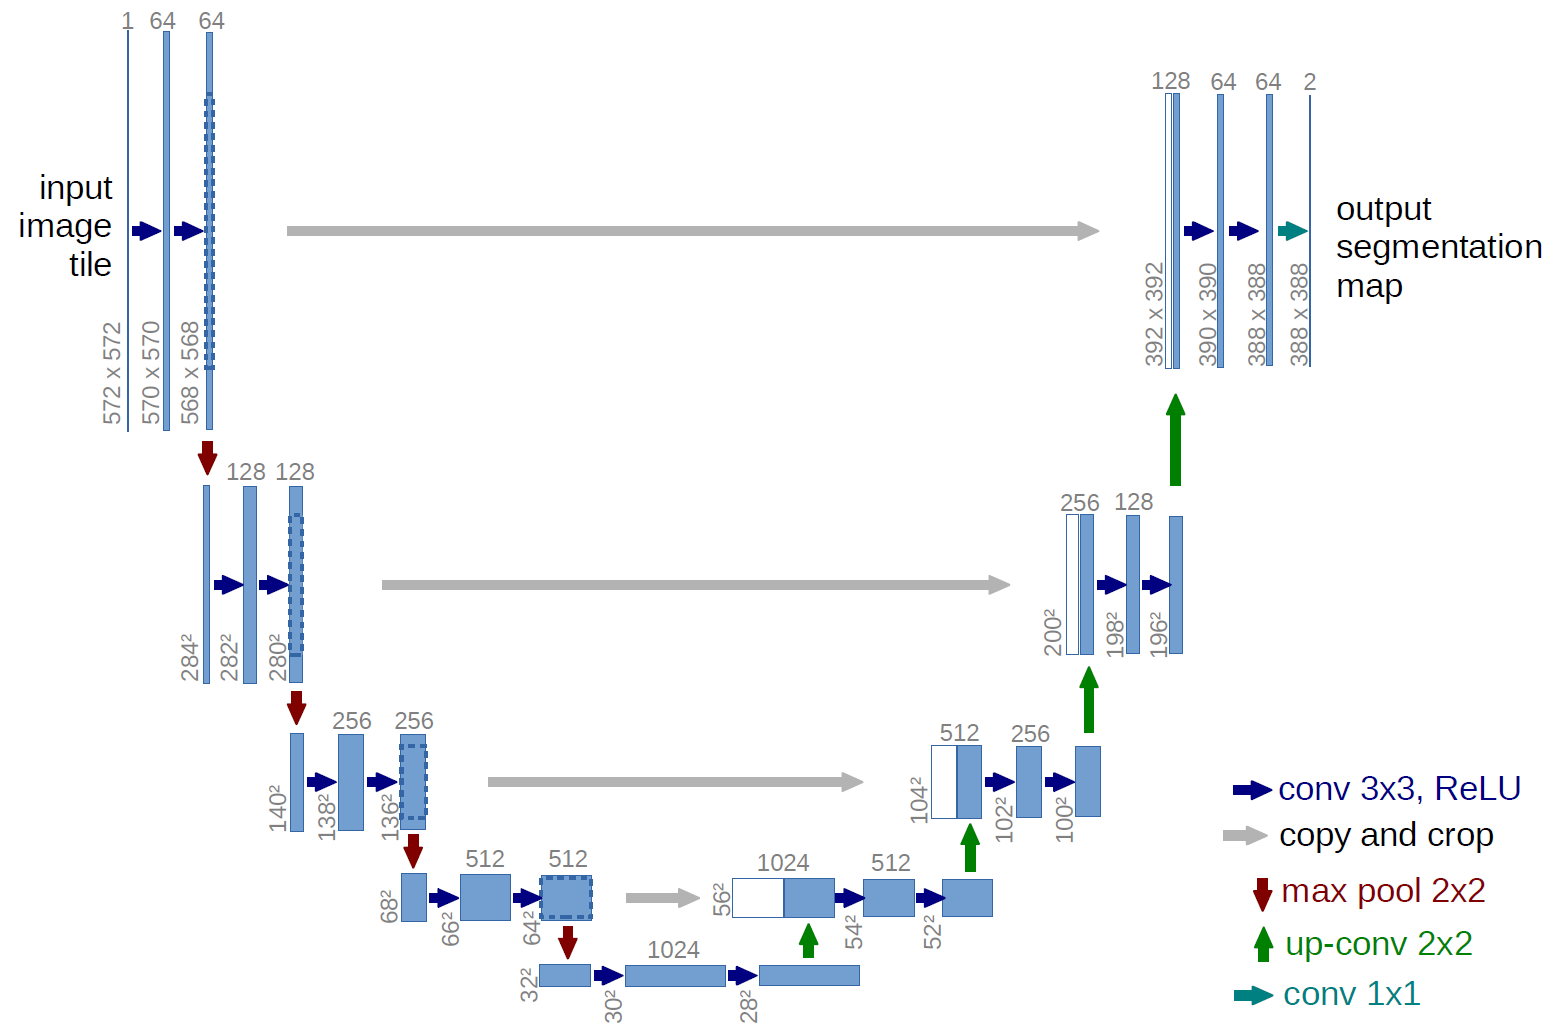
\includegraphics[width=\textwidth]{images/unet.png}
\captionof{figure}{U-Net model}
\end{center}



% TODO: U-Net
% -> PyEDDL
% -> Tensorflow
%
% -> Dice scores
% -> Profiling
% -> Network output

\newpage
\section{Double U-Net}
Start writing about Double U-Net.

% TODO: Describe the model
% TODO: Training parameters

\begin{center}
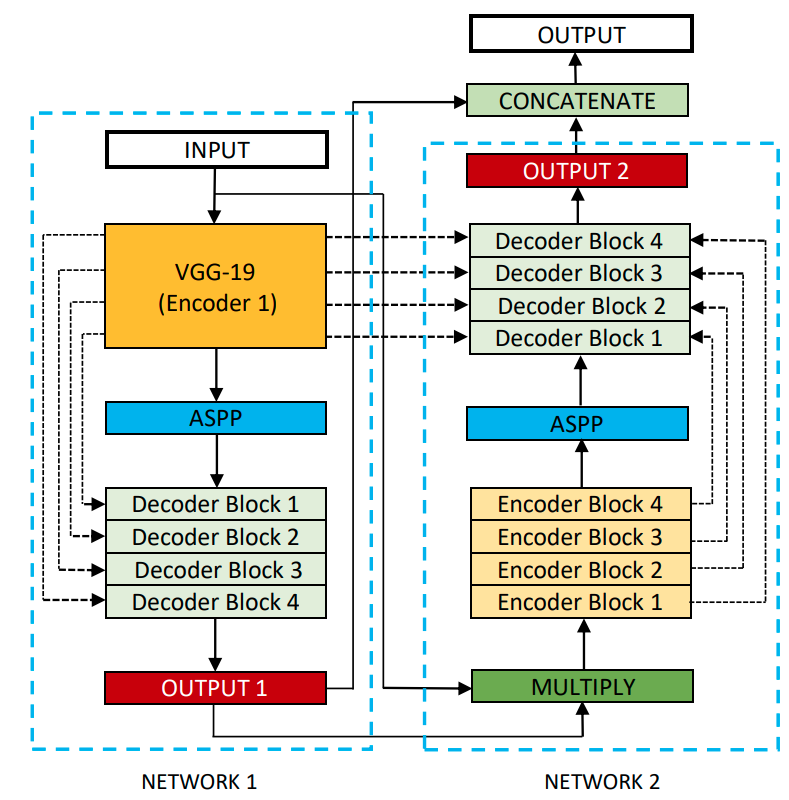
\includegraphics[width=\textwidth]{images/double_unet.png}
\captionof{figure}{Double U-Net model}
\end{center}
% TODO: Double U-Net
% -> PyEDDL
% -> Tensorflow
%
% -> Dice scores
% -> Profiles
% -> Network output

% \section{Comparison}